\documentclass[11pt]{article}\usepackage[]{graphicx}\usepackage[]{color}
%% maxwidth is the original width if it is less than linewidth
%% otherwise use linewidth (to make sure the graphics do not exceed the margin)
\makeatletter
\def\maxwidth{ %
  \ifdim\Gin@nat@width>\linewidth
    \linewidth
  \else
    \Gin@nat@width
  \fi
}
\makeatother

\definecolor{fgcolor}{rgb}{0.345, 0.345, 0.345}
\newcommand{\hlnum}[1]{\textcolor[rgb]{0.686,0.059,0.569}{#1}}%
\newcommand{\hlstr}[1]{\textcolor[rgb]{0.192,0.494,0.8}{#1}}%
\newcommand{\hlcom}[1]{\textcolor[rgb]{0.678,0.584,0.686}{\textit{#1}}}%
\newcommand{\hlopt}[1]{\textcolor[rgb]{0,0,0}{#1}}%
\newcommand{\hlstd}[1]{\textcolor[rgb]{0.345,0.345,0.345}{#1}}%
\newcommand{\hlkwa}[1]{\textcolor[rgb]{0.161,0.373,0.58}{\textbf{#1}}}%
\newcommand{\hlkwb}[1]{\textcolor[rgb]{0.69,0.353,0.396}{#1}}%
\newcommand{\hlkwc}[1]{\textcolor[rgb]{0.333,0.667,0.333}{#1}}%
\newcommand{\hlkwd}[1]{\textcolor[rgb]{0.737,0.353,0.396}{\textbf{#1}}}%

\usepackage{framed}
\makeatletter
\newenvironment{kframe}{%
 \def\at@end@of@kframe{}%
 \ifinner\ifhmode%
  \def\at@end@of@kframe{\end{minipage}}%
  \begin{minipage}{\columnwidth}%
 \fi\fi%
 \def\FrameCommand##1{\hskip\@totalleftmargin \hskip-\fboxsep
 \colorbox{shadecolor}{##1}\hskip-\fboxsep
     % There is no \\@totalrightmargin, so:
     \hskip-\linewidth \hskip-\@totalleftmargin \hskip\columnwidth}%
 \MakeFramed {\advance\hsize-\width
   \@totalleftmargin\z@ \linewidth\hsize
   \@setminipage}}%
 {\par\unskip\endMakeFramed%
 \at@end@of@kframe}
\makeatother

\definecolor{shadecolor}{rgb}{.97, .97, .97}
\definecolor{messagecolor}{rgb}{0, 0, 0}
\definecolor{warningcolor}{rgb}{1, 0, 1}
\definecolor{errorcolor}{rgb}{1, 0, 0}
\newenvironment{knitrout}{}{} % an empty environment to be redefined in TeX

\usepackage{alltt}
\usepackage{amsmath}
\usepackage{listings}
\usepackage{stmaryrd}
\usepackage{bbm}
\usepackage{amsmath}
\usepackage{mathtools}
\usepackage{pdfpages}
\usepackage{breqn}
\usepackage[utf8]{inputenc}


\newcount\colveccount
\newcommand*\colvec[1]{
        \global\colveccount#1
        \begin{pmatrix}
        \colvecnext
}
\def\colvecnext#1{
        #1
        \global\advance\colveccount-1
        \ifnum\colveccount>0
                \\
                \expandafter\colvecnext
        \else
                \end{pmatrix}
        \fi
}
\newcommand{\argmin}{\arg\!\min}

\author{Thibault Doutre, Student ID 26980469}
\title{STAT230 HW 11 \\
University of California, Berkeley}
\date{\today}
\IfFileExists{upquote.sty}{\usepackage{upquote}}{}
\begin{document}

\maketitle
\section{Orthonormal variables}
I first generate the data with standard independent normal variables.
\begin{knitrout}
\definecolor{shadecolor}{rgb}{0.969, 0.969, 0.969}\color{fgcolor}\begin{kframe}
\begin{alltt}
\hlstd{makedata}\hlkwb{=}\hlkwa{function}\hlstd{(}\hlkwc{p}\hlstd{=}\hlnum{20}\hlstd{,}\hlkwc{n}\hlstd{=}\hlnum{100}\hlstd{)\{}
  \hlstd{X}\hlkwb{=}\hlkwd{matrix}\hlstd{(}\hlkwd{rnorm}\hlstd{(n}\hlopt{*}\hlstd{p),n,p)}
  \hlstd{exps}\hlkwb{=}\hlkwd{seq}\hlstd{(}\hlopt{-}\hlnum{1}\hlstd{,}\hlopt{-}\hlnum{2.5}\hlstd{,}\hlkwc{length}\hlstd{=p)}
  \hlstd{beta}\hlkwb{=}\hlkwd{rep}\hlstd{(}\hlnum{0}\hlstd{,p)}
  \hlstd{beta}\hlkwb{=}\hlkwd{exp}\hlstd{(exps)}
  \hlstd{Y}\hlkwb{=}\hlnum{.5}\hlopt{+}\hlstd{X}\hlopt\hlstd{beta}\hlopt{+}\hlkwd{rnorm}\hlstd{(n)}
  \hlstd{data} \hlkwb{=} \hlkwd{data.frame}\hlstd{(Y,X)}
  \hlkwd{colnames}\hlstd{(data)}\hlkwb{=}\hlkwd{c}\hlstd{(}\hlstr{"Y"}\hlstd{,letters[}\hlnum{1}\hlopt{:}\hlnum{20}\hlstd{])}
  \hlstd{switch}\hlkwb{=}\hlkwd{sample}\hlstd{(}\hlnum{20}\hlstd{)}\hlopt{+}\hlnum{1}
  \hlstd{data}\hlkwb{=}\hlstd{data[,}\hlkwd{c}\hlstd{(}\hlnum{1}\hlstd{,switch)]}
  \hlkwd{names}\hlstd{(beta)}\hlkwb{=}\hlkwd{names}\hlstd{(data)[switch]}
  \hlkwd{return}\hlstd{(data)}
\hlstd{\}}
\end{alltt}
\end{kframe}
\end{knitrout}
Then, I set a bunch of functions. Each of them computes a tenfolded cross validation of the method they use. The output is binary: $y$ corresponds to the $MSE$, averaged over the 10 folds and $x$ corresponds to the degree of freedom, which depends on the method used.
\begin{itemize}
\item $cv_ols$ performs backward selection based on the t-value, with fitting an OLS method every time. The degrees of freedom are defined as the number of variables taken into the model.
\item $cv_pcr$ performs PCR. The degrees of freedom are again defined as the number of variables taken into the model.
\item $cv_tree$ performs tree pruning after having fitted a tree model to the data. The degrees of freedom is defined as the size of the tree, i.e. the number of terminal nodes.
\item $cv_ridge$ performs ridge regression. The degrees of freedom are defined as $-\log{\lambda}$ where $\lambda$ is the shrinkage coefficient. I then map this value to the 0-20 range in order to compare this method with the others.
\item $cv_lasso$ performs lasso regression. The degrees of freedom are defined as the number of non zero weights in front of the coefficients.
\end{itemize}
\begin{knitrout}
\definecolor{shadecolor}{rgb}{0.969, 0.969, 0.969}\color{fgcolor}\begin{kframe}
\begin{alltt}
\hlcom{## # PCR}
\hlkwd{library}\hlstd{(pls)}
\end{alltt}


{\ttfamily\noindent\itshape\color{messagecolor}{\#\# \\\#\# Attaching package: 'pls'}}

{\ttfamily\noindent\itshape\color{messagecolor}{\#\# The following object is masked from 'package:stats':\\\#\# \\\#\#\ \ \ \  loadings}}\begin{alltt}
\hlstd{cv_pcr} \hlkwb{=} \hlkwa{function}\hlstd{(}\hlkwc{data}\hlstd{)\{}
  \hlstd{p} \hlkwb{=} \hlkwd{ncol}\hlstd{(data)}\hlopt{-}\hlnum{1}
  \hlstd{pcr.fit} \hlkwb{=} \hlkwd{pcr}\hlstd{(Y}\hlopt{~}\hlnum{0}\hlopt{+}\hlstd{.,} \hlkwc{ncomp}\hlstd{=p,} \hlkwc{data}\hlstd{=data,} \hlkwc{validation} \hlstd{=}\hlstr{"CV"}\hlstd{)}
  \hlstd{cv_error} \hlkwb{=} \hlkwd{as.data.frame}\hlstd{(}\hlkwd{RMSEP}\hlstd{(pcr.fit)}\hlopt{$}\hlstd{val)[}\hlnum{1}\hlstd{,]}
  \hlkwd{names}\hlstd{(cv_error)} \hlkwb{=} \hlnum{0}\hlopt{:}\hlstd{p}
  \hlkwd{return}\hlstd{(}\hlkwd{list}\hlstd{(}\hlkwc{y}\hlstd{=cv_error,}\hlkwc{x}\hlstd{=}\hlkwd{rev}\hlstd{(}\hlnum{0}\hlopt{:}\hlstd{p)))}
\hlstd{\}}

\hlcom{## # OLS}
\hlstd{cv_ols_one} \hlkwb{=} \hlkwa{function}\hlstd{(}\hlkwc{data}\hlstd{,} \hlkwc{nfold}\hlstd{=}\hlnum{10}\hlstd{,} \hlkwc{formula}\hlstd{=}\hlstr{"Y~."}\hlstd{)\{}
  \hlstd{Y_cv} \hlkwb{=} \hlkwd{c}\hlstd{()}
  \hlstd{nrows} \hlkwb{=} \hlkwd{nrow}\hlstd{(data)}
  \hlstd{MSE_test} \hlkwb{=} \hlkwd{c}\hlstd{()}
  \hlkwa{for} \hlstd{(i} \hlkwa{in} \hlkwd{seq}\hlstd{(}\hlnum{0}\hlstd{, nrows}\hlopt{-}\hlstd{nfold,} \hlkwc{by}\hlstd{=nrows}\hlopt{/}\hlstd{nfold))\{}
    \hlstd{test} \hlkwb{=} \hlstd{(i}\hlopt{+}\hlnum{1}\hlstd{)}\hlopt{:}\hlstd{(nfold}\hlopt{+}\hlstd{i)}
    \hlstd{train} \hlkwb{=} \hlopt{-}\hlstd{test}
    \hlstd{lm.fit} \hlkwb{=} \hlkwd{lm}\hlstd{(formula,} \hlkwc{data}\hlstd{=data[train,])}
    \hlstd{Ytest} \hlkwb{=} \hlkwd{predict}\hlstd{(lm.fit, data[test,])}
    \hlstd{MSE_test} \hlkwb{=} \hlkwd{c}\hlstd{(MSE_test,} \hlkwd{mean}\hlstd{((data}\hlopt{$}\hlstd{Y[test]}\hlopt{-}\hlstd{Ytest)}\hlopt{^}\hlnum{2}\hlstd{))}
  \hlstd{\}}
  \hlkwd{return}\hlstd{(}\hlkwd{mean}\hlstd{(MSE_test))}
\hlstd{\}}
\hlstd{cv_ols} \hlkwb{=} \hlkwa{function}\hlstd{(}\hlkwc{data}\hlstd{)\{}
  \hlstd{p}\hlkwb{=}\hlkwd{ncol}\hlstd{(data)}\hlopt{-}\hlnum{1}
  \hlstd{nfold}\hlkwb{=}\hlnum{10}
  \hlstd{formula} \hlkwb{=} \hlstr{"Y~."}
  \hlstd{lm.fit} \hlkwb{=} \hlkwd{lm}\hlstd{(formula,} \hlkwc{data}\hlstd{=data)}
  \hlstd{MSE_test} \hlkwb{=} \hlkwd{c}\hlstd{()}
  \hlstd{next_to_remove} \hlkwb{=} \hlstr{""}
  \hlstd{variables} \hlkwb{=} \hlkwd{c}\hlstd{()}
  \hlstd{n} \hlkwb{=} \hlkwd{nrow}\hlstd{(data)}
  \hlkwa{while}\hlstd{(}\hlkwd{length}\hlstd{(}\hlkwd{names}\hlstd{(lm.fit}\hlopt{$}\hlstd{model))}\hlopt{>}\hlnum{1}\hlstd{)\{}
    \hlstd{MSE} \hlkwb{=} \hlkwd{cv_ols_one}\hlstd{(data,} \hlkwc{nfold}\hlstd{=nfold, formula)}
    \hlstd{MSE_test} \hlkwb{=} \hlkwd{c}\hlstd{(MSE,MSE_test)}
    \hlstd{t_values} \hlkwb{=} \hlkwd{coef}\hlstd{(}\hlkwd{summary}\hlstd{(lm.fit))[,}\hlstr{"t value"}\hlstd{]}
    \hlstd{next_to_remove} \hlkwb{=} \hlkwd{names}\hlstd{(}\hlkwd{which.min}\hlstd{(t_values[}\hlopt{-}\hlnum{1}\hlstd{]))}
    \hlstd{variables} \hlkwb{=} \hlkwd{c}\hlstd{(next_to_remove,variables)}
    \hlstd{formula} \hlkwb{=} \hlkwd{paste}\hlstd{(formula,}\hlstr{"-"}\hlstd{,next_to_remove,}\hlkwc{sep}\hlstd{=}\hlstr{""}\hlstd{)}
    \hlstd{lm.fit} \hlkwb{=} \hlkwd{update}\hlstd{(lm.fit, formula)}
  \hlstd{\}}
  \hlstd{MSE} \hlkwb{=} \hlkwd{cv_ols_one}\hlstd{(data, nfold, formula)}
  \hlstd{MSE_test} \hlkwb{=} \hlkwd{c}\hlstd{(MSE,MSE_test)}
  \hlkwd{return}\hlstd{(}\hlkwd{list}\hlstd{(}\hlkwc{y}\hlstd{=MSE_test,}\hlkwc{x}\hlstd{=}\hlnum{0}\hlopt{:}\hlstd{p))}
\hlstd{\}}


\hlcom{## # Tree}
\hlkwd{library}\hlstd{(tree)}
\hlstd{cv_tree} \hlkwb{<-} \hlkwa{function}\hlstd{(}\hlkwc{a}\hlstd{)\{}
  \hlkwd{assign}\hlstd{(}\hlstr{"a"}\hlstd{, a, .GlobalEnv)}
  \hlstd{tree.out}\hlkwb{=}\hlkwd{tree}\hlstd{(Y}\hlopt{~}\hlnum{1}\hlopt{+}\hlstd{.,} \hlkwc{data}\hlstd{=a)}
  \hlstd{cv} \hlkwb{=} \hlkwd{cv.tree}\hlstd{(tree.out)}
  \hlstd{MSE} \hlkwb{=} \hlstd{cv}\hlopt{$}\hlstd{dev}\hlopt{/}\hlnum{100}
  \hlstd{size} \hlkwb{=} \hlnum{20}\hlopt{-}\hlstd{cv}\hlopt{$}\hlstd{size}
  \hlstd{y}\hlkwb{=}\hlkwd{rep}\hlstd{(}\hlnum{NaN}\hlstd{,}\hlnum{21}\hlstd{)}
  \hlstd{y[size]}\hlkwb{=}\hlstd{MSE}
  \hlkwd{return}\hlstd{(}\hlkwd{list}\hlstd{(}\hlkwc{y}\hlstd{=y,}\hlkwc{x}\hlstd{=}\hlnum{0}\hlopt{:}\hlnum{20}\hlstd{))}
\hlstd{\}}


\hlcom{## # Ridge}
\hlkwd{library}\hlstd{(glmnet)}
\end{alltt}


{\ttfamily\noindent\itshape\color{messagecolor}{\#\# Loading required package: Matrix}}

{\ttfamily\noindent\itshape\color{messagecolor}{\#\# Loading required package: foreach}}

{\ttfamily\noindent\itshape\color{messagecolor}{\#\# Loaded glmnet 2.0-2}}\begin{alltt}
\hlstd{cv_ridge} \hlkwb{=} \hlkwa{function}\hlstd{(}\hlkwc{data}\hlstd{)\{}
  \hlstd{x} \hlkwb{=} \hlkwd{as.matrix}\hlstd{(data[,}\hlopt{-}\hlnum{1}\hlstd{])}
  \hlstd{y} \hlkwb{=} \hlstd{data[,}\hlnum{1}\hlstd{]}
  \hlstd{cv.out} \hlkwb{=} \hlkwd{cv.glmnet}\hlstd{(x,y,}\hlkwc{alpha}\hlstd{=}\hlnum{0}\hlstd{,}\hlkwc{type.measure}\hlstd{=}\hlstr{"mse"}\hlstd{)}
  \hlstd{MSE} \hlkwb{=} \hlstd{cv.out}\hlopt{$}\hlstd{cvm}
  \hlstd{lambda} \hlkwb{=} \hlstd{cv.out}\hlopt{$}\hlstd{lambda}
  \hlstd{m} \hlkwb{=} \hlopt{-}\hlkwd{log}\hlstd{(lambda)}
  \hlstd{mapped_m} \hlkwb{=} \hlstd{(m}\hlopt{-}\hlkwd{min}\hlstd{(m))}\hlopt{/}\hlstd{(}\hlkwd{max}\hlstd{(m)}\hlopt{-}\hlkwd{min}\hlstd{(m))}\hlopt{*}\hlnum{20}
  \hlstd{df} \hlkwb{=} \hlkwd{data.frame}\hlstd{(}\hlkwc{mse}\hlstd{=MSE,}\hlkwc{mapped_m}\hlstd{=}\hlkwd{as.integer}\hlstd{(mapped_m))}
  \hlstd{y}\hlkwb{=}\hlkwd{c}\hlstd{()}
  \hlkwa{for} \hlstd{(i} \hlkwa{in} \hlnum{0}\hlopt{:}\hlnum{20}\hlstd{)\{}
    \hlstd{ind} \hlkwb{=} \hlkwd{which}\hlstd{(df}\hlopt{$}\hlstd{mapped_m}\hlopt{==}\hlstd{i)}
    \hlstd{y}\hlkwb{=}\hlkwd{c}\hlstd{(y,}\hlkwd{mean}\hlstd{(df}\hlopt{$}\hlstd{mse[ind]))}
  \hlstd{\}}
  \hlkwd{return} \hlstd{(}\hlkwd{list}\hlstd{(}\hlkwc{y}\hlstd{=y,}\hlkwc{x}\hlstd{=}\hlkwd{unique}\hlstd{(df}\hlopt{$}\hlstd{mapped_m) ))}
\hlstd{\}}


\hlcom{## # Lasso}
\hlstd{cv_lasso} \hlkwb{=} \hlkwa{function}\hlstd{(}\hlkwc{data}\hlstd{)\{}
  \hlstd{x} \hlkwb{=} \hlkwd{as.matrix}\hlstd{(data[,}\hlopt{-}\hlnum{1}\hlstd{])}
  \hlstd{y} \hlkwb{=} \hlstd{data[,}\hlnum{1}\hlstd{]}
  \hlstd{cv.out} \hlkwb{=} \hlkwd{cv.glmnet}\hlstd{(x,y,}\hlkwc{alpha}\hlstd{=}\hlnum{1}\hlstd{,}\hlkwc{type.measure}\hlstd{=}\hlstr{"mse"}\hlstd{)}
  \hlstd{MSE} \hlkwb{=} \hlstd{cv.out}\hlopt{$}\hlstd{cvm}
  \hlstd{deg} \hlkwb{=} \hlstd{cv.out}\hlopt{$}\hlstd{nzero}
  \hlstd{df} \hlkwb{=} \hlkwd{data.frame}\hlstd{(}\hlkwc{mse}\hlstd{=MSE,}\hlkwc{deg}\hlstd{=deg)}
  \hlstd{y}\hlkwb{=}\hlkwd{c}\hlstd{()}
  \hlkwa{for} \hlstd{(i} \hlkwa{in} \hlnum{0}\hlopt{:}\hlnum{20}\hlstd{)\{}
    \hlstd{ind} \hlkwb{=} \hlkwd{which}\hlstd{(df}\hlopt{$}\hlstd{deg}\hlopt{==}\hlstd{i)}
    \hlstd{y}\hlkwb{=}\hlkwd{c}\hlstd{(y,}\hlkwd{mean}\hlstd{(df}\hlopt{$}\hlstd{mse[ind]))}
  \hlstd{\}}
  \hlkwd{return} \hlstd{(}\hlkwd{list}\hlstd{(}\hlkwc{y}\hlstd{=y,}\hlkwc{x}\hlstd{=}\hlkwd{unique}\hlstd{(deg)))}
\hlstd{\}}
\end{alltt}
\end{kframe}
\end{knitrout}
Now, I write a plot function in order to see the difference performances of the methods used. Basically I compute the different methods $B$ times and then I compute the means and the standard errors of the distributions of the cross validated errors for each model. I parallelize everything in order to make it much faster. Hoever, I do not parallelize the tree method for a little difficulty I don't want to extend myself on.
\begin{knitrout}
\definecolor{shadecolor}{rgb}{0.969, 0.969, 0.969}\color{fgcolor}\begin{kframe}
\begin{alltt}
\hlkwd{library}\hlstd{(parallel)}
\hlstd{plot_cv} \hlkwb{=} \hlkwa{function}\hlstd{(}\hlkwc{method}\hlstd{,} \hlkwc{B}\hlstd{=}\hlnum{100}\hlstd{,} \hlkwc{same_y} \hlstd{=} \hlnum{FALSE}\hlstd{)\{}
  \hlstd{data} \hlkwb{=} \hlkwd{makedata}\hlstd{()}
  \hlkwa{if} \hlstd{(method}\hlopt{==}\hlstr{"Tree"}\hlstd{)\{}
    \hlstd{CV}\hlkwb{=}\hlkwd{t}\hlstd{(}\hlkwd{sapply}\hlstd{(}\hlnum{1}\hlopt{:}\hlstd{B,} \hlkwa{function}\hlstd{(}\hlkwc{i}\hlstd{,}\hlkwc{...}\hlstd{)}
    \hlstd{\{a}\hlkwb{=}\hlkwd{cv_tree}\hlstd{(data)}\hlopt{$}\hlstd{y;}\hlkwd{return}\hlstd{(a)\}))}
  \hlstd{\}}
  \hlkwa{else}\hlstd{\{}
    \hlstd{ncores} \hlkwb{=} \hlkwd{detectCores}\hlstd{()}\hlopt{-}\hlnum{1}
    \hlstd{cl} \hlkwb{=} \hlkwd{makeCluster}\hlstd{(ncores)}
    \hlkwd{clusterEvalQ}\hlstd{(cl,}\hlkwd{c}\hlstd{(}\hlkwd{library}\hlstd{(pls),}\hlkwd{library}\hlstd{(glmnet),}\hlkwd{library}\hlstd{(tree)))}
    \hlkwd{clusterExport}\hlstd{(cl,}\hlkwd{list}\hlstd{(}\hlstr{"makedata"}\hlstd{,}\hlstr{"cv_pcr"}\hlstd{,}
                          \hlstr{"cv_tree"}\hlstd{,}\hlstr{"cv_ridge"}\hlstd{,}\hlstr{"cv_ols"}\hlstd{,}
                          \hlstr{"cv_lasso"}\hlstd{,}\hlstr{"cv_ols_one"}\hlstd{,}\hlstr{"glmnet"}\hlstd{))}

    \hlkwa{if} \hlstd{(method}\hlopt{==}\hlstr{"PCR"}\hlstd{)\{R} \hlkwb{=} \hlkwd{parSapply}\hlstd{(cl,} \hlnum{1}\hlopt{:}\hlstd{B,} \hlkwa{function}\hlstd{(}\hlkwc{i}\hlstd{,}\hlkwc{...}\hlstd{)}
    \hlstd{\{a}\hlkwb{=}\hlkwd{cv_pcr}\hlstd{(data)}\hlopt{$}\hlstd{y;} \hlkwd{return}\hlstd{(a)\})\}}
    \hlkwa{if} \hlstd{(method}\hlopt{==}\hlstr{"Lasso"}\hlstd{)\{R} \hlkwb{=} \hlkwd{parSapply}\hlstd{(cl,} \hlnum{1}\hlopt{:}\hlstd{B,} \hlkwa{function}\hlstd{(}\hlkwc{i}\hlstd{,}\hlkwc{...}\hlstd{)}
    \hlstd{\{a}\hlkwb{=}\hlkwd{cv_lasso}\hlstd{(data)}\hlopt{$}\hlstd{y;} \hlkwd{return}\hlstd{(a)\})\}}
    \hlkwa{if} \hlstd{(method}\hlopt{==}\hlstr{"Ridge"}\hlstd{)\{R} \hlkwb{=} \hlkwd{parSapply}\hlstd{(cl,} \hlnum{1}\hlopt{:}\hlstd{B,} \hlkwa{function}\hlstd{(}\hlkwc{i}\hlstd{,}\hlkwc{...}\hlstd{)}
    \hlstd{\{a}\hlkwb{=}\hlkwd{cv_ridge}\hlstd{(data)}\hlopt{$}\hlstd{y;} \hlkwd{return}\hlstd{(a)\})\}}
    \hlkwa{if} \hlstd{(method}\hlopt{==}\hlstr{"OLS"}\hlstd{)\{R} \hlkwb{=} \hlkwd{parSapply}\hlstd{(cl,} \hlnum{1}\hlopt{:}\hlstd{B,} \hlkwa{function}\hlstd{(}\hlkwc{i}\hlstd{,}\hlkwc{...}\hlstd{)}
    \hlstd{\{a}\hlkwb{=}\hlkwd{cv_ols}\hlstd{(data)}\hlopt{$}\hlstd{y;} \hlkwd{return}\hlstd{(a)\})\}}

    \hlstd{CV} \hlkwb{=} \hlkwd{matrix}\hlstd{(}\hlkwd{unlist}\hlstd{(R),} \hlkwc{nrow} \hlstd{= B,} \hlkwc{byrow} \hlstd{= T)}
    \hlkwd{stopCluster}\hlstd{(cl)}
  \hlstd{\}}

  \hlstd{avg} \hlkwb{=} \hlkwd{apply}\hlstd{(CV,}\hlnum{2}\hlstd{,}\hlkwa{function}\hlstd{(}\hlkwc{x}\hlstd{)\{}
    \hlkwa{if} \hlstd{(}\hlkwd{all}\hlstd{(}\hlkwd{is.nan}\hlstd{(x)))\{}\hlnum{NA}\hlstd{\}}
    \hlkwa{else}\hlstd{\{}\hlkwd{mean}\hlstd{(x[}\hlopt{!}\hlkwd{is.nan}\hlstd{(x)])\}\})}
  \hlstd{se} \hlkwb{=} \hlkwd{apply}\hlstd{(CV,}\hlnum{2}\hlstd{,}\hlkwa{function}\hlstd{(}\hlkwc{x}\hlstd{)\{}
    \hlkwa{if} \hlstd{(}\hlkwd{all}\hlstd{(}\hlkwd{is.nan}\hlstd{(x)))\{}\hlnum{NA}\hlstd{\}}
    \hlkwa{else}\hlstd{\{}\hlkwd{sd}\hlstd{(x[}\hlopt{!}\hlkwd{is.nan}\hlstd{(x)])\}\})}
  \hlkwa{if} \hlstd{(same_y)\{}
    \hlkwd{plot}\hlstd{(avg,}\hlkwc{ylim}\hlstd{=}\hlkwd{c}\hlstd{(}\hlnum{0.8}\hlstd{,}\hlnum{2}\hlstd{),}
         \hlkwc{xlab}\hlstd{=}\hlstr{"df"}\hlstd{,}\hlkwc{ylab}\hlstd{=}\hlstr{"CV error"}\hlstd{,}\hlkwc{main}\hlstd{=method)}
  \hlstd{\}}
  \hlkwa{else}\hlstd{\{}
    \hlkwd{plot}\hlstd{(avg,}\hlkwc{ylim}\hlstd{=}\hlkwd{c}\hlstd{(}\hlkwd{min}\hlstd{(avg}\hlopt{-}\hlstd{se,}\hlkwc{na.rm} \hlstd{= T),}\hlkwd{max}\hlstd{(avg}\hlopt{+}\hlstd{se,}\hlkwc{na.rm} \hlstd{= T)),}
         \hlkwc{xlab}\hlstd{=}\hlstr{"df"}\hlstd{,}\hlkwc{ylab}\hlstd{=}\hlstr{"CV error"}\hlstd{,}\hlkwc{main}\hlstd{=method)}
  \hlstd{\}}
  \hlkwd{points}\hlstd{(avg}\hlopt{+}\hlstd{se,}\hlkwc{col}\hlstd{=}\hlstr{"darkgrey"}\hlstd{,}\hlkwc{pch}\hlstd{=}\hlnum{2}\hlstd{)}
  \hlkwd{points}\hlstd{(avg}\hlopt{-}\hlstd{se,}\hlkwc{col}\hlstd{=}\hlstr{"darkgrey"}\hlstd{,}\hlkwc{pch}\hlstd{=}\hlnum{2}\hlstd{)}
  \hlkwd{abline}\hlstd{(}\hlkwc{h} \hlstd{=} \hlkwd{min}\hlstd{(avg}\hlopt{+}\hlstd{se,}\hlkwc{na.rm} \hlstd{= T),} \hlkwc{lty} \hlstd{=} \hlnum{2}\hlstd{,} \hlkwc{col}\hlstd{=}\hlstr{"darkgrey"}\hlstd{)}
\hlstd{\}}
\end{alltt}
\end{kframe}
\end{knitrout}

\begin{knitrout}
\definecolor{shadecolor}{rgb}{0.969, 0.969, 0.969}\color{fgcolor}\begin{kframe}
\begin{alltt}
\hlcom{# Different scales}
\hlkwd{par}\hlstd{(}\hlkwc{mfrow}\hlstd{=}\hlkwd{c}\hlstd{(}\hlnum{2}\hlstd{,}\hlnum{3}\hlstd{),}\hlkwc{oma}\hlstd{=}\hlkwd{c}\hlstd{(}\hlnum{0}\hlstd{,}\hlnum{0}\hlstd{,}\hlnum{3}\hlstd{,}\hlnum{0}\hlstd{))}
\hlkwd{plot_cv}\hlstd{(}\hlstr{"Tree"}\hlstd{)}
\hlkwd{plot_cv}\hlstd{(}\hlstr{"OLS"}\hlstd{)}
\hlkwd{plot_cv}\hlstd{(}\hlstr{"PCR"}\hlstd{)}
\hlkwd{plot_cv}\hlstd{(}\hlstr{"Ridge"}\hlstd{)}
\hlkwd{plot_cv}\hlstd{(}\hlstr{"Lasso"}\hlstd{)}
\hlkwd{title}\hlstd{(}\hlstr{"MSE based on different methods"}\hlstd{,}\hlkwc{outer}\hlstd{=T)}
\hlkwd{par}\hlstd{(}\hlkwc{mfrow}\hlstd{=}\hlkwd{c}\hlstd{(}\hlnum{1}\hlstd{,}\hlnum{1}\hlstd{))}
\end{alltt}
\end{kframe}
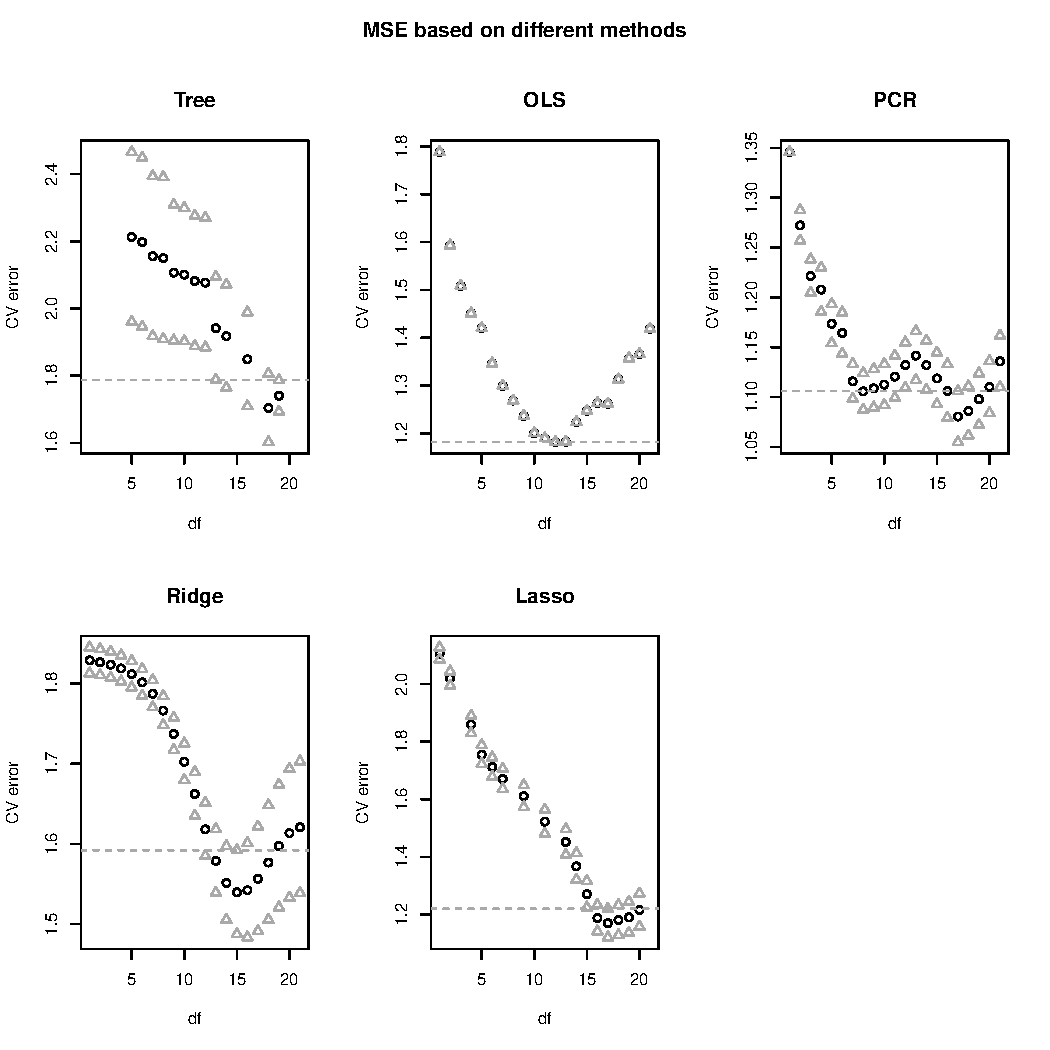
\includegraphics[width=\maxwidth]{figure/unnamed-chunk-4-1} 

\end{knitrout}

OLS won because of the data generating process. The data satisfies the OLS assumptions, i.e the orthogonality of the variables. We can see that the best model is for $df$ around 10. However, for the trees, df=20 gives the best model. This is because trees have a very low bias (but a high variance). They perform poorly compared to the other methods here. The ridge regression and the lasso perform well here, although the L2 penalty here (ridge) gives better results than the L1 (lasso) because since the data is gaussian, it makes more sense to maximize the posterior with a gaussian prior than a double exponential prior.

\section{Correlated explanatory variables}
I change the $makedata$ function in order to have correlated explanatory variables.
\begin{knitrout}
\definecolor{shadecolor}{rgb}{0.969, 0.969, 0.969}\color{fgcolor}\begin{kframe}
\begin{alltt}
\hlkwd{rm}\hlstd{(makedata)}

\hlstd{gen_corr} \hlkwb{=} \hlkwa{function}\hlstd{(}\hlkwc{n} \hlstd{=} \hlnum{100}\hlstd{,}
                    \hlkwc{r} \hlstd{=} \hlnum{0.05}\hlstd{,}
                    \hlkwc{n_replications} \hlstd{=} \hlnum{3}\hlstd{)\{}
  \hlstd{G} \hlkwb{=} \hlkwd{matrix}\hlstd{(r,n,n)} \hlopt{+} \hlkwd{diag}\hlstd{(}\hlnum{1}\hlopt{-}\hlstd{r,n,n)}
  \hlstd{chol_G} \hlkwb{=} \hlkwd{chol}\hlstd{(G)}
  \hlstd{epsilons} \hlkwb{=} \hlkwd{matrix}\hlstd{(}\hlkwd{rnorm}\hlstd{(n}\hlopt{*}\hlstd{n_replications),n,n_replications)}
  \hlstd{epsilons} \hlkwb{=} \hlkwd{as.data.frame}\hlstd{(chol_G} \hlopt \hlstd{epsilons)}
  \hlkwd{return}\hlstd{(epsilons)}
\hlstd{\}}

\hlstd{makedata} \hlkwb{=} \hlkwa{function}\hlstd{(}\hlkwc{n}\hlstd{=}\hlnum{100}\hlstd{,}\hlkwc{p}\hlstd{=}\hlnum{20}\hlstd{)\{}
  \hlstd{data1} \hlkwb{=} \hlkwd{gen_corr}\hlstd{(}\hlkwc{r}\hlstd{=}\hlnum{.1}\hlstd{,} \hlkwc{n}\hlstd{=}\hlnum{100}\hlstd{)}
  \hlstd{data2} \hlkwb{=} \hlkwd{gen_corr}\hlstd{(}\hlkwc{r}\hlstd{=}\hlnum{.3}\hlstd{,} \hlkwc{n}\hlstd{=}\hlnum{100}\hlstd{)}
  \hlstd{data3} \hlkwb{=} \hlkwd{gen_corr}\hlstd{(}\hlkwc{r}\hlstd{=}\hlnum{.5}\hlstd{,} \hlkwc{n}\hlstd{=}\hlnum{100}\hlstd{)}
  \hlstd{data4} \hlkwb{=} \hlkwd{gen_corr}\hlstd{(}\hlkwc{r}\hlstd{=}\hlnum{.7}\hlstd{,} \hlkwc{n}\hlstd{=}\hlnum{100}\hlstd{)}
  \hlstd{data5} \hlkwb{=} \hlkwd{gen_corr}\hlstd{(}\hlkwc{r}\hlstd{=}\hlnum{.9}\hlstd{,} \hlkwc{n}\hlstd{=}\hlnum{100}\hlstd{)}
  \hlstd{data6} \hlkwb{=} \hlkwd{matrix}\hlstd{(}\hlkwd{rnorm}\hlstd{(}\hlnum{5}\hlopt{*}\hlstd{n),}\hlkwc{ncol}\hlstd{=}\hlnum{5}\hlstd{,} \hlkwc{nrow}\hlstd{=n)}
  \hlstd{X} \hlkwb{=} \hlkwd{as.matrix}\hlstd{(}\hlkwd{cbind}\hlstd{(data1,data2,data3,data4,}
               \hlstd{data5,data6))}
  \hlkwd{names}\hlstd{(X)} \hlkwb{=} \hlnum{1}\hlopt{:}\hlnum{20}
  \hlstd{exps}\hlkwb{=}\hlkwd{seq}\hlstd{(}\hlopt{-}\hlnum{1}\hlstd{,}\hlopt{-}\hlnum{2.5}\hlstd{,}\hlkwc{length}\hlstd{=p)}
  \hlstd{beta}\hlkwb{=}\hlkwd{rep}\hlstd{(}\hlnum{0}\hlstd{,p)}
  \hlstd{beta}\hlkwb{=}\hlkwd{exp}\hlstd{(exps)}
  \hlstd{Y}\hlkwb{=}\hlnum{.5}\hlopt{+}\hlstd{X}\hlopt\hlstd{beta}\hlopt{+}\hlkwd{rnorm}\hlstd{(n)}
  \hlstd{data} \hlkwb{=} \hlkwd{data.frame}\hlstd{(Y,X)}
  \hlkwd{colnames}\hlstd{(data)}\hlkwb{=}\hlkwd{c}\hlstd{(}\hlstr{"Y"}\hlstd{,letters[}\hlnum{1}\hlopt{:}\hlnum{20}\hlstd{])}
  \hlstd{switch}\hlkwb{=}\hlkwd{sample}\hlstd{(}\hlnum{20}\hlstd{)}\hlopt{+}\hlnum{1}
  \hlstd{data}\hlkwb{=}\hlstd{data[,}\hlkwd{c}\hlstd{(}\hlnum{1}\hlstd{,switch)]}
  \hlkwd{names}\hlstd{(beta)}\hlkwb{=}\hlkwd{names}\hlstd{(data)[switch]}
  \hlkwd{return}\hlstd{(data)}
\hlstd{\}}
\end{alltt}
\end{kframe}
\end{knitrout}
If we make the explanatory variables correlated, the OLS assumptions are no longer true. 

\begin{knitrout}
\definecolor{shadecolor}{rgb}{0.969, 0.969, 0.969}\color{fgcolor}\begin{kframe}
\begin{alltt}
\hlcom{# Different scales}
\hlkwd{par}\hlstd{(}\hlkwc{mfrow}\hlstd{=}\hlkwd{c}\hlstd{(}\hlnum{2}\hlstd{,}\hlnum{3}\hlstd{),}\hlkwc{oma}\hlstd{=}\hlkwd{c}\hlstd{(}\hlnum{0}\hlstd{,}\hlnum{0}\hlstd{,}\hlnum{3}\hlstd{,}\hlnum{0}\hlstd{))}
\hlkwd{plot_cv}\hlstd{(}\hlstr{"Tree"}\hlstd{)}
\hlkwd{plot_cv}\hlstd{(}\hlstr{"OLS"} \hlstd{)}
\hlkwd{plot_cv}\hlstd{(}\hlstr{"PCR"} \hlstd{)}
\hlkwd{plot_cv}\hlstd{(}\hlstr{"Ridge"}\hlstd{)}
\hlkwd{plot_cv}\hlstd{(}\hlstr{"Lasso"}\hlstd{)}
\hlkwd{title}\hlstd{(}\hlstr{"MSE based on different methods"}\hlstd{,}\hlkwc{outer}\hlstd{=T)}
\hlkwd{par}\hlstd{(}\hlkwc{mfrow}\hlstd{=}\hlkwd{c}\hlstd{(}\hlnum{1}\hlstd{,}\hlnum{1}\hlstd{))}
\end{alltt}
\end{kframe}
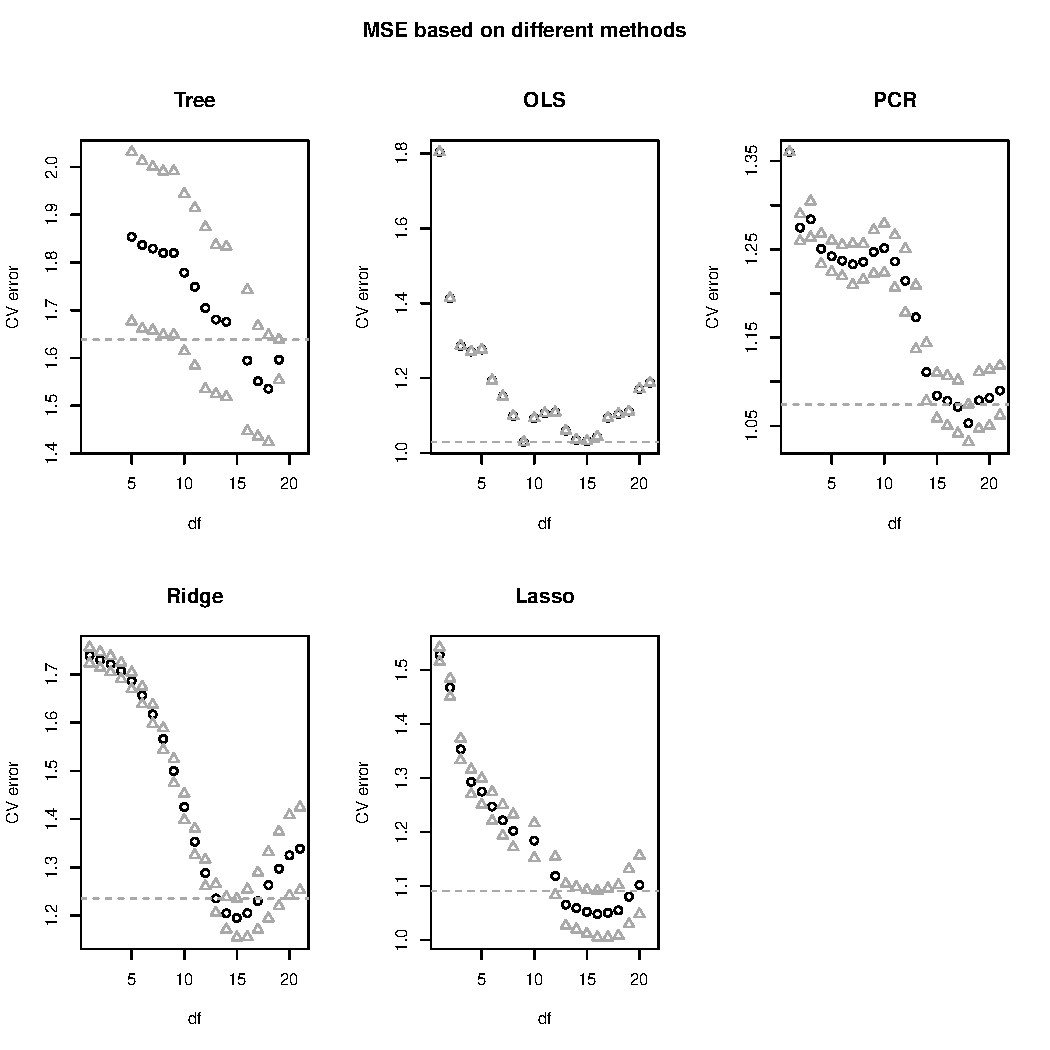
\includegraphics[width=\maxwidth]{figure/unnamed-chunk-6-1} 

\end{knitrout}

\section{Discussion}
A few commments:
\begin{itemize}
\item 1 - In the first simulation, the backward selection with OLS do have the best results since the data is generated with 20 independent random variables, and this satisfies the OLS assumption. In the second simulation, PCR behaves better than OLS since the variables are not orthogonal. Indeed, the orthogonalization of the features force the OLS assumptions to be true. 
\item 2 - Ridge regression shrinks all directions, but unlike lasso it does not explicitely set any variable to be zero. Lasso has a heavy penalty here compared to ridge and OLS. In OLS, the variables kept are the orthogonal ones, i.e. the 5 orthogonal generated at the end of the data set and the 5 others which have nothing to do with the other. In Ridge we keep almost all of them and in Lasso the best $df$ is around 5.
\item 3 - Principal components regression only takes some orthogonal components to do the regression, and discards the rest. In other words it only takes some components of the orthonormalized basis of the feature set. Lasso applies a L1 penalty and Ridge a L2 penalty. The L1 penalty tends to shrink the feature coefficients to exactly zero. On the other hand, Ridge will include all the $p$ features in the model.
\item 4 - For tree based method it is very different. Since the trees have a very low bias, the more the features the better. However, the splits strongly depend on the data set, which means they have high variance. This is why they behave poorly. In order to reduce the variance of the algorithm, we can take i.i.d versions of trees by bootstrapping the set of features before fitting a tree and then averaging over all the trees: this leads to random forests.
\end{itemize}


\end{document}









